\documentclass{article}
\usepackage[utf8]{inputenc}
\usepackage[T1]{fontenc}
\usepackage{lmodern}
\usepackage{geometry}
\usepackage{graphicx}
\usepackage{hyperref}
\usepackage{enumitem}
\usepackage{amsmath}
\usepackage{amssymb}
\geometry{margin=1in}

\title{AA arte de los algoritmos}
\date{}

\begin{document}
\maketitle
\tableofcontents
\newpage

\section{Explicar problema}
\begin{figure}[h]
\centering
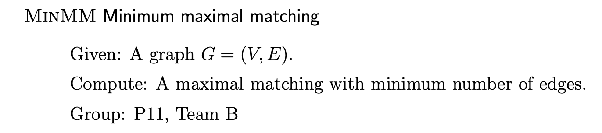
\includegraphics[width=0.8\linewidth]{images/image1.png}
\end{figure}
((A \textbf{maximal matching} is a matching \textit{M} of a graph \textit{G} that is not a subset of any other matching. A matching \textit{M} of a graph \textit{G} is maximal if every edge in \textit{G} has a non-empty intersection with at least one edge in \textit{M}. The following figure shows examples of maximal matchings (red) in three graphs.))

Un \textbf{maximal matching} és un matching M d'un graf G que no és un subset de cap altre matching. Un matching M d'un graf G és maximal si cada aresta en G té una intersecció no buida amb com a mínim una aresta de M. La següent figura mostra matchings maximals (vermell) en tres grafs [1]:
\begin{figure}[h]
\centering
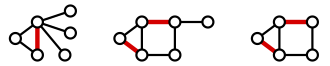
\includegraphics[width=0.8\linewidth]{images/image2.png}
\end{figure}

Un minimal maximal matching és un matching M de G tal que no hi ha cap altre matching amb menor nombre d'arestes.

Propietats:

Un maximal matching M de tamany k per a un graf G és també un edge dominating set de tamany k per a G.
Un edge dominating set és per a un graf G un subset D de les arestes tal que cada aresta fora de D és adjacent a una aresta en D. [2]
\begin{figure}[h]
\centering
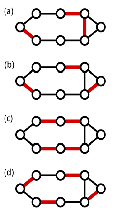
\includegraphics[width=0.8\linewidth]{images/image3.png}
\end{figure}
Busquem minimitzar-ho, per tant, obtenir el conjunt D de mida k mínima tq es forma un dominating set. No hi haura cap subconjunt D de mida k-1 tq siqui un maximal matching, i tota aresta no pertanyent a D sigui adjaceny a una aresta en D.
El problema decisional de trobar un dominating set de tamany k és equivalent al de trobar un maximal matching de tamany k. Aquest problema és també un problema conegut per ser NP-Complet, i la seva versió de minimització NP-Dificil. L'equivalència d'aquests dos problemes ens ajuda a reforçar la complexitat de minimum maximal matching.

\section{Explicar complexitat problema}
Tot i que el problema de maximal matching es pot resoldre en temps polinòmic, no es coneix cap algoritme de temps polinòmic per resoldre minimum maximal matching.
El problema decisional de trobar un maximal matching amb tamany k és un exemple clar de un problema NP-Complet, I per tant el problema d'optimització de trobar el seu mínim és NP-Hard d'Optimització.

Veurem la prova que és NP-hard amb una reducció de Vertex Cover (un altre problema NP-hard).
Explicació de Vertex Cover:
	Donat un graf $G = \{V,E\}$
	Me devuelve un conjunto de vertices C tq toda arista del grafo tiene un extremo en un vertice del conjunto C.
Reducció:
	Partim de la Idea que si tenim un Vertex Cover, no podem treure cap node per cobrir totes les aristes.
	Partim d'un graf G i generarem un G' tq:

\begin{itemize}
	\item Per tota arista $(u,v) \in E$ en generem un node $X_{uv}$
\item Afegim només les aristes entre u i Xuv, i v i Xuv.
\item (Tota arista pasa a ser un vertex.)
\end{itemize}

Com construir el Matching desde G'?

\begin{itemize}
	\item Aparello tot node $X_{uv}$ amb un node $\in C$ (al vertex cover).
\item Això em dona un aparellament maximal (no puc afegir cap i minim, tmp ho puc fer en menys).
	\item Sempre, si tinc un vertex cover de $k$ nodes, tindré un aparellament amb $k' \le |E| + k \rightarrow$ puc acotar el nombre d'aparellaments reduint la $k$ del vertex cover.
\end{itemize}

	Per que funciona?

\begin{itemize}
\item Aquest aparellament cobreix els nodes corresponents mitjançant els vèrtexs Xuv, i és maximal ja que no es poden afegir més arestes sense violar les restriccions. També serà minim ja que mai no es podrà fer amb un nombre menor d'arestes.
\item La importància darrera l'optimització del VC és que a menor VC, se'ns garanteix que podrem trobar un MinMM menor (acotat millor) i fer-ho més optim.
\item Desd el meu G' puc tornar a VC agafant els vertexs aparellats a G'
\end{itemize}

La NP-Dificultat de MinMM esta reforçada per la seva dificultat en varis subproblemes. Esta demostrat que MinMM és NP-dificil per a grafs bipartits amb grau maxim 3, grafs planars bipartits i grafs planars cubics i grafs bipartits k-regulars per a qualevol $k \ge 3$, entre altres.

Tot i aixo hi ha alguns casos per als que MMM es pot resoldre en temps polinomic per a arbres, arbres de cliques (block graph) i altres casos que es veuran a continuació.
És tambe conegut que el tamany d'un maximal matching no pot ser mai major que el doble del minimum maximal matching d'un graph. Per tant, qualsevol algoritme per trobar un maximal matching pot obtenir una 2-aproximació per a MinMM.

\section{Explicar complexitat de subproblemes trobats}
MinMM es NP-Dificil en grafs bipartits regulars

La complexitat de MinMM pot variar segons les caracterìstiques del graf. Quan es busca demostrar la complexitat d'aquest problema es sol avaluar per a subproblemes concrets.

Per als següents subproblemes la complexitat de MinMM està demostrada com a NP-dificil:

\textbf{Grafs Bipartits} amb grau màxim 3.[3]
Un graf bipartit és un graf G tal que els seus vertex es poden dividir en dos sets disjunts i independents U i V. Cada aresta connecta un vertex de U a un de V. [4]

\textbf{Grafs Plans} amb grau màxim 3.[3]
Un graf pla és un graf tal que pot ser dibuixat en un pla sense que les arestes s'intersequin.[5]

\textbf{Grafs Quasi-Regulars}[3]
Un graf quasi-regular és un graf tal que el rang entre el grau mínim i el grau màxim està acotat.

\textbf{Grafs Regulars} amb una k fixa $\ge 3$ [3]
Un graf regular és un graf tal que el grau de cada vertex és igual

\textbf{Grafs Bipartits k-regulars} [3]

Minimum Maximal \textbf{Induced} Matching [9]

Minimum Maximal \textbf{Acyclic} Matching

Minimum Maximal \textbf{Uniquely Restricted} Matching
Un matching induït és un matching M per a un graf G tal que les arestes en M són les úniques arestes en G que connecten qualsevols vertex u,v tal que una aresta en M els conté.
Si eliminem en G les arestes de M, la distancia entre qualsevol parell de vèrtex en M és com a mínim 2.

Per als següents subproblemes és coneixen algorismes polinòmics per a MinMM:

\textbf{Grafs Regulars} amb una k = 2 [3]
\textbf{Arbres} [3]
Un arbre és un graf connex acíclic no dirigit.

\textbf{Arbre de cliques} [3]
Un arbre de cliques és un tipus de graf no dirigit en el que cada component biconnectat és un clique.[6]

\textbf{Graf sèrie-paral·lel} [3]
Un graf serie-paral·lel és un graf amb dos vertex expecials denominats com a terminals. Aquests grafs es construeixen recursivament mitjançant operacions de composició en sèrie o en paral·lel.[7]
\begin{figure}[h]
\centering
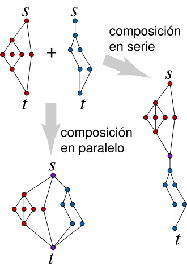
\includegraphics[width=0.8\linewidth]{images/image4.png}
\end{figure}
\textbf{Graf permutació bipartit} [3]
Un graf permutació és un graf tal que els seus vertex representen els elements d'una seqüència i les arestes representen parells d'elements revertits en una permutació concreta de la seqüència.[8]

\section{Algoritmes d’aproximacio}
Tots els algoritmes d’aproximació pasen per el fet que qualsevol maximal matching es com a maxim 2 cops mes gran que el minimum maximal matching.

\subsection{Demostracio (tot maximal matching es una 2-aproximacio del minimum maximal matching)}


\section{Algoritmes aleatoris}
\href{https://doi.org/10.1080/00207160.2013.853052}{https://doi.org/10.1080/00207160.2013.853052}
\href{https://doi.org/10.1016/j.disopt.2007.11.010}{https://doi.org/10.1016/j.disopt.2007.11.010}

\href{https://en.wikipedia.org/wiki/Block\_graph}{Block graph - Wikipedia}

Referencies:

\begin{enumerate}
\item Wikipedia contributors. (2025, May 18). Matching (graph theory). In \textit{Wikipedia, The Free Encyclopedia}. Retrieved March 23, 2026, from \href{https://en.wikipedia.org/wiki/Matching\\\_(graph\\\_theory}{https://en.wikipedia.org/wiki/Matching\\\_(graph\\\_theory}
\item Wikipedia contributors. (2024, May 14). Edge dominating set. In \textit{Wikipedia, The Free Encyclopedia}. Retrieved March 23, 2026, from \href{https://en.wikipedia.org/wiki/Edge\\\_dominating\\\_set}{https://en.wikipedia.org/wiki/Edge\\\_dominating\\\_set}
\item Demange, M., Ekim, T., \& Ries, B. (2014). Hardness and approximation of minimum maximal matching. \textit{International Journal of Computer Mathematics}, \textit{91}(8), 1737--1752. \href{https://doi.org/10.1080/00207160.2013.853052}{https://doi.org/10.1080/00207160.2013.853052}
\item Wikipedia contributors. (2026, March 14). Bipartite graph. In \textit{Wikipedia, The Free Encyclopedia}. Retrieved March 23, 2026, from \href{https://en.wikipedia.org/wiki/Bipartite\\\_graph}{https://en.wikipedia.org/wiki/Bipartite\\\_graph}
\item Wikipedia contributors. (2026, March 5). Planar graph. In \textit{Wikipedia, The Free Encyclopedia}. Retrieved March 23, 2026, from \href{https://en.wikipedia.org/wiki/Planar\\\_graph}{https://en.wikipedia.org/wiki/Planar\\\_graph}
\item Wikipedia contributors. (2026, February 16). Block graph. In \textit{Wikipedia, The Free Encyclopedia}. Retrieved March 24, 2026, from \href{https://en.wikipedia.org/wiki/Block\\\_graph}{https://en.wikipedia.org/wiki/Block\\\_graph}
\item Wikipedia contributors. (2025, diciembre 22). Grafo serie-paralelo. En \textit{Wikipedia, La enciclopedia libre}. Recuperado el 24 de marzo de 2026, de \href{https://es.wikipedia.org/wiki/Grafo\\\_serie-paralelo}{https://es.wikipedia.org/wiki/Grafo\\\_serie-paralelo}
\item Wikipedia contributors. (2026, February 20). Permutation graph. In \textit{Wikipedia, The Free Encyclopedia}. Retrieved March 24, 2026, from \href{https://en.wikipedia.org/wiki/Permutation\\\_graph}{https://en.wikipedia.org/wiki/Permutation\\\_graph}
\item Cameron, I. D., \& Canoy, M. S. (2008). Minimum maximal matching in chordal graphs. \textit{Discrete Applied Optimization}, \textit{5}(2), 121--130. \href{https://doi.org/10.1016/j.disopt.2007.11.010}{https://doi.org/10.1016/j.disopt.2007.11.010}
\item Wikipedia contributors. (2025, November 12). Induced matching. In \textit{Wikipedia, The Free Encyclopedia}. Retrieved March 25, 2026, from \href{https://en.wikipedia.org/wiki/Induced\\\_matching}{https://en.wikipedia.org/wiki/Induced\\\_matching}
\end{enumerate}

Complexitat problemes decisionals edge dominating set i MinMM:

\begin{enumerate}
\item \href{https://en.wikipedia.org/wiki/Michael\\\_R.\\\_Garey}{Garey, Michael R.}; \href{https://en.wikipedia.org/wiki/David\\\_S.\\\_Johnson}{Johnson, David S.} (1979), \href{https://en.wikipedia.org/wiki/Computers\\\_and\\\_Intractability:\\\_A\\\_Guide\\\_to\\\_the\\\_Theory\\\_of\\\_NP-Completeness}{\textit{Computers and Intractability: A Guide to the Theory of NP-Completeness}}, W.H. Freeman, \href{https://en.wikipedia.org/wiki/ISBN\\\_(identifier}{ISBN}) \href{https://en.wikipedia.org/wiki/Special:BookSources/0-7167-1045-5}{0-7167-1045-5}. Edge dominating set (decision version) is discussed under the dominating set problem, which is the problem GT2 in Appendix A1.1. Minimum maximal matching (decision version) is the problem GT10 in Appendix A1.1.
\item Yannakakis, M., y F. Gavril. «Edge Dominating Sets in Graphs». \textit{SIAM Journal on Applied Mathematics}, vol. 38, n.o 3, junio de 1980, pp. 364-72. \textit{DOI.org (Crossref)}, https://doi.org/10.1137/0138030.
\end{enumerate}

Aplicacions:

\begin{enumerate}
\item AlMeshari, Khalid A., et al. “Innovative Strategies in Kidney Paired Donation: Single-Center Experience Achieving the Highest Annual Transplant Volume Globally.” \textit{Frontiers in Immunology}, vol. 17, p. 1623684. \textit{PubMed Central}, https://doi.org/10.3389/fimmu.2026.1623684. Accessed 27 Mar. 2026.
\end{enumerate}

\textbf{2-aproximación (caso general)}

\textbf{Algoritmo: (Versión 2, misma explicación (2-aprox) que si los elijo aleatorios completamente, y el coste si que mejora, no uso heap, cojo uno random)}

\begin{enumerate}
\item Mientras haya aristas en el grafo
\item Selecciona la arista cuyos extremos tengan \textbf{mayor suma de grados}
\item Añádela al matching
\item Elimina ambos extremos y todas sus aristas incidentes
\item Actualiza los grados
\end{enumerate}

\textbf{Correcto?} Sí, me da Matching

\textbf{Coste?}

Utilizamos: lista de adyacencia + cola de prioridad (max-heap) sobre grados.

Cada iteración:

\textit{ Extraer la arista de mayor grado del heap: \textbf{O(log |E|)}
} Eliminar los dos extremos y sus aristas incidentes: \textbf{$O(\Delta)$} donde $\Delta$ es el grado máximo
\begin{itemize}
\item Actualizar grados de vecinos afectados en el heap: \textbf{$O(\Delta \cdot \log |E|)$}
\end{itemize}

Como cada arista se elimina como máximo una vez en todo el algoritmo, el trabajo total de eliminaciones es \textbf{O(|E|)}. Por tanto:

\[
T(n)=O(|E|\cdot\log|E|)
\]

\textbf{Aproximación: (donde el optimo es el MinMM y yo obtengo un MM)}

\begin{figure}[h]
\centering
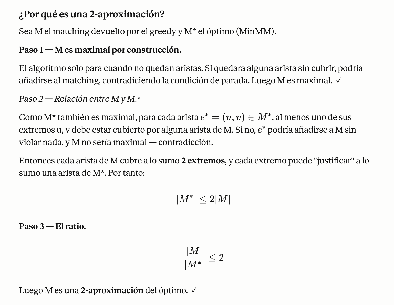
\includegraphics[width=0.8\linewidth]{images/image5.png}
\end{figure}

\href{https://arxiv.org/pdf/1811.08506}{https://arxiv.org/pdf/1811.08506}

\textbf{Connected Cubic graph}
(2518+O(1n))-approximation algorithm for minimum maximal matching in connected cubic graphs.
Que es un connected cubic graph?
Todos los vertices tienen exactamente 3 conexiones, y es conexo.

\href{https://www.combinatorics.org/ojs/index.php/eljc/article/view/v29i2p36/pdf}{https://www.combinatorics.org/ojs/index.php/eljc/article/view/v29i2p36/pdf}


\end{document}
